\documentclass[10pt,a4paper]{article}

\usepackage[margin=1.7cm]{geometry}
\usepackage{graphicx}
\usepackage{booktabs}
\usepackage{amsmath}
\usepackage{float}
\usepackage[hidelinks]{hyperref}
\setlength{\parindent}{0pt}
\setlength{\parskip}{5pt}

\begin{document}

% Page 1
\begin{titlepage}
\centering
\vspace*{2.2cm}
{\LARGE\bfseries Thermochemical Performance Study of a N2O/Paraffin Hybrid Rocket Motor Using Cantera\par}
\vspace{1cm}
{\large Computer Methods in Combustion\par}
{\large Metody komputerowe w spalaniu\par}
\vspace{1.8cm}
\begin{tabular}{ll}
\toprule
Author & Szymon Krupa \\
Coordinator & dr inz. Mateusz Zbikowski \\
Project type & Python / Cantera thermochemical analysis \\
Propellant pair & N2O / paraffin fuel surrogate (C2H4) \\
Number of pages & 9 \\
Date & June 2026 \\
\bottomrule
\end{tabular}
\vfill
\textbf{Repository}\par
\url{https://github.com/szymonkrupa78/MKWS_2026_Krupa_Szymon}
\end{titlepage}

% Page 2
\section*{Abstract}
This project presents a reproducible Python/Cantera study of an idealized nitrous oxide/paraffin hybrid rocket motor. The solid paraffin grain is represented by ethylene (C2H4), a gas-phase surrogate for hydrocarbon pyrolysis products available in GRI-Mech 3.0. The model combines constant-pressure adiabatic equilibrium calculations with ideal frozen-gamma nozzle relations and an illustrative single-port fuel-regression model.

The analysis evaluates oxidizer-to-fuel mass ratios from 3.0 to 12.0 and chamber pressures from 10 to 80 bar. The main outputs are equilibrium chamber temperature, product composition, heat-capacity ratio, mean molecular weight, transport properties, characteristic velocity, sea-level and vacuum specific impulse, and a time history of the fuel port. The highest characteristic velocity at 20 bar is obtained at O/F = 5.25, while maximum ideal vacuum specific impulse occurs at O/F = 5.50. Both values are strongly fuel-rich compared with the stoichiometric O/F of 9.41.

\subsection*{Project Deliverables}
\begin{itemize}
\item reusable thermochemistry, nozzle, and internal-ballistics code;
\item generated CSV result tables and figures;
\item five numerical and physical-consistency tests;
\item a reproducible LaTeX and PDF technical report.
\end{itemize}

\subsection*{Contents}
\begin{tabular}{clc}
\toprule
Section & Title & Page \\
\midrule
1 & Introduction and State of the Art & 2 \\
2 & Model Description & 3 \\
3 & Program Description and Verification & 4 \\
4 & O/F Sweep Results & 5 \\
5 & Rocket Performance Results & 6 \\
6 & Pressure and Transport Results & 7 \\
7 & Hybrid Port Regression, Limitations, Conclusions & 8 \\
\bottomrule
\end{tabular}
\newpage

% Page 3
\section{Introduction}
A hybrid rocket motor stores the fuel and oxidizer in different physical phases. In the configuration considered here, the fuel is a solid hydrocarbon grain with a cylindrical port, while nitrous oxide is delivered through the port as the oxidizer. The separated propellants provide operational advantages: the motor can be shut down by stopping oxidizer flow, the solid fuel is comparatively simple to store, and the architecture uses fewer fluid systems than a bipropellant liquid engine.

Hybrid combustion is coupled to internal ballistics. Oxidizer mass flux controls the regression rate of the fuel surface. As the port grows, oxidizer flux, fuel mass flow, mixture ratio, chamber conditions, and thrust can all change. Thermochemistry and grain geometry therefore cannot be selected independently.

\subsection{Objective}
The objective is to create a transparent computational tool for preliminary reasoning about a N2O/paraffin motor. The project asks which O/F range gives the best ideal performance, how chamber pressure changes the predicted state and nozzle performance, and how a simple port-regression law moves the motor through the O/F map during an eight-second burn.

\subsection{State of the Art}
Chemical equilibrium is a standard first step in rocket analysis. NASA CEA and similar tools minimize thermodynamic potentials subject to elemental conservation to estimate product composition and theoretical performance. Cantera solves the same class of equilibrium problem and exposes thermodynamic and transport properties through a Python API.

Detailed hybrid prediction would require multiphase flow, heat transfer into the grain, melting and entrainment of paraffin, surface pyrolysis, finite-rate mixing, injector behavior, and a validated regression correlation. The present work remains at a preliminary level: gas-phase equilibrium for the chamber, frozen-gamma nozzle equations, and a power-law regression model. These assumptions make trends easy to interpret but prevent the model from serving as final hardware design evidence.
\newpage

% Page 4
\section{Model Description}
\subsection{Reactant Composition}
The oxidizer is N2O and the fuel vapor is represented by C2H4. Ethylene is not a complete physical model of paraffin; it is a gas-phase surrogate with an approximate CH2 elemental ratio and is available together with N2O chemistry in \texttt{gri30.yaml}. For a one-kilogram fuel basis:
\[
n_f = \frac{1}{M_f}, \qquad n_{ox} = \frac{O/F}{M_{ox}}.
\]
The global stoichiometric relation is
\[
\mathrm{C_2H_4 + 6N_2O \rightarrow 2CO_2 + 2H_2O + 6N_2},
\]
which gives stoichiometric O/F = 9.41.

\subsection{Equilibrium Chamber State}
Reactants enter at 298.15 K. Cantera solves an adiabatic constant-pressure equilibrium problem:
\[
h(T,p,Y)=h_{initial}, \qquad p=p_{chamber}.
\]
The code records temperature, density, $c_p$, $c_v$, heat-capacity ratio, mean molecular weight, specific gas constant, sound speed, viscosity, thermal conductivity, Prandtl number, and selected product mole fractions.

\subsection{Ideal Nozzle Model}
The nozzle uses a fixed expansion area ratio $A_e/A_t=15$. Chamber $\gamma$ and gas constant are frozen during expansion. The exit Mach number is found by inverting the area-Mach relation. Characteristic velocity is
\[
c^*=\sqrt{\frac{RT_c}{\gamma}}
\left(\frac{\gamma+1}{2}\right)^{\frac{\gamma+1}{2(\gamma-1)}}.
\]
Momentum and pressure-thrust terms give sea-level and vacuum thrust coefficients, followed by $I_{sp}=c^*C_F/g_0$.
\newpage

% Page 5
\section{Program Description and Verification}
The repository separates physical calculations, plotting, orchestration, tests, data, and the report.

\begin{tabular}{p{5.4cm}p{10.1cm}}
\toprule
Path & Responsibility \\
\midrule
\texttt{src/mkws\_hybrid/thermochemistry.py} & Equilibrium, gas properties, area-Mach inversion, nozzle performance \\
\texttt{src/mkws\_hybrid/hybrid\_model.py} & Single cylindrical port and regression history \\
\texttt{src/mkws\_hybrid/plotting.py} & Plots and report summary panel \\
\texttt{scripts/run\_study.py} & Sweeps, CSV export, and figures \\
\texttt{scripts/make\_report\_pdf.py} & PDF generation \\
\texttt{tests/test\_thermochemistry.py} & Unit and physical-consistency tests \\
\bottomrule
\end{tabular}

\subsection{Reproduction}
\begin{verbatim}
python -m venv .venv
source .venv/bin/activate
pip install -r requirements.txt
python scripts/run_study.py
python -m unittest discover -s tests
python scripts/make_report_pdf.py
\end{verbatim}

\subsection{Tests}
\begin{tabular}{lll}
\toprule
Test & Purpose & Result \\
\midrule
Stoichiometric O/F & N2O/C2H4 molecular-weight ratio & PASS \\
Mass O/F conversion & Requested oxidizer/fuel mass ratio & PASS \\
Area-Mach inverse & Supersonic branch at area ratio 15 & PASS \\
Physical chamber case & T, gamma, c*, Isp, Prandtl ranges & PASS \\
Port regression & Increasing diameter and O/F drift & PASS \\
\bottomrule
\end{tabular}
\newpage

% Page 6
\section{O/F Sweep Results}
The adiabatic temperature increases rapidly from fuel-rich conditions and reaches approximately 3383 K near O/F = 7.50 at 20 bar. Increasing pressure raises equilibrium temperature because dissociation is suppressed. The detailed temperature maximum remains below stoichiometric O/F = 9.41.

\begin{figure}[H]
\centering
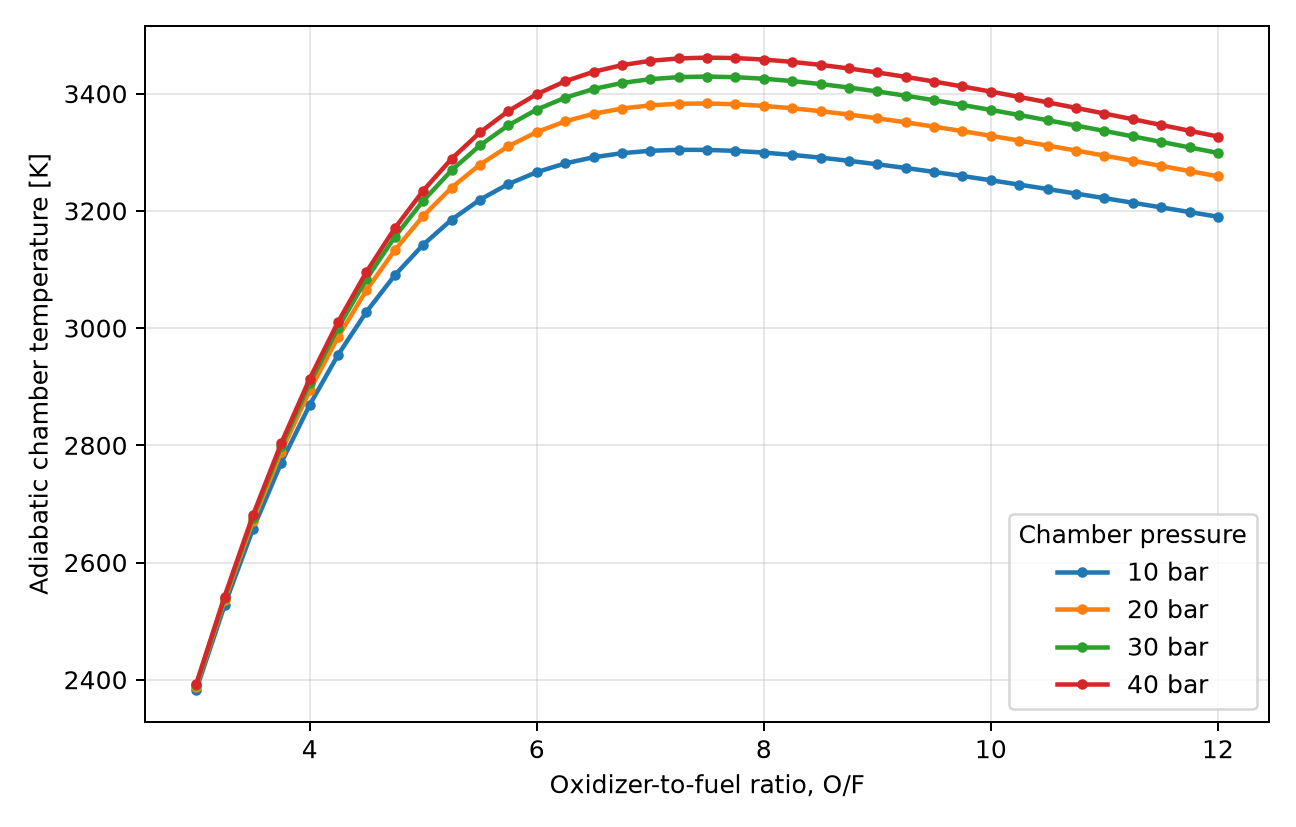
\includegraphics[width=0.82\linewidth]{../figures/adiabatic_temperature_vs_of.png}
\caption{Adiabatic equilibrium chamber temperature versus O/F for four chamber pressures.}
\end{figure}

Low O/F gives high CO and H2 fractions. Moving toward stoichiometric conditions increases H2O and CO2, while NO becomes more important at high temperature.

\begin{figure}[H]
\centering
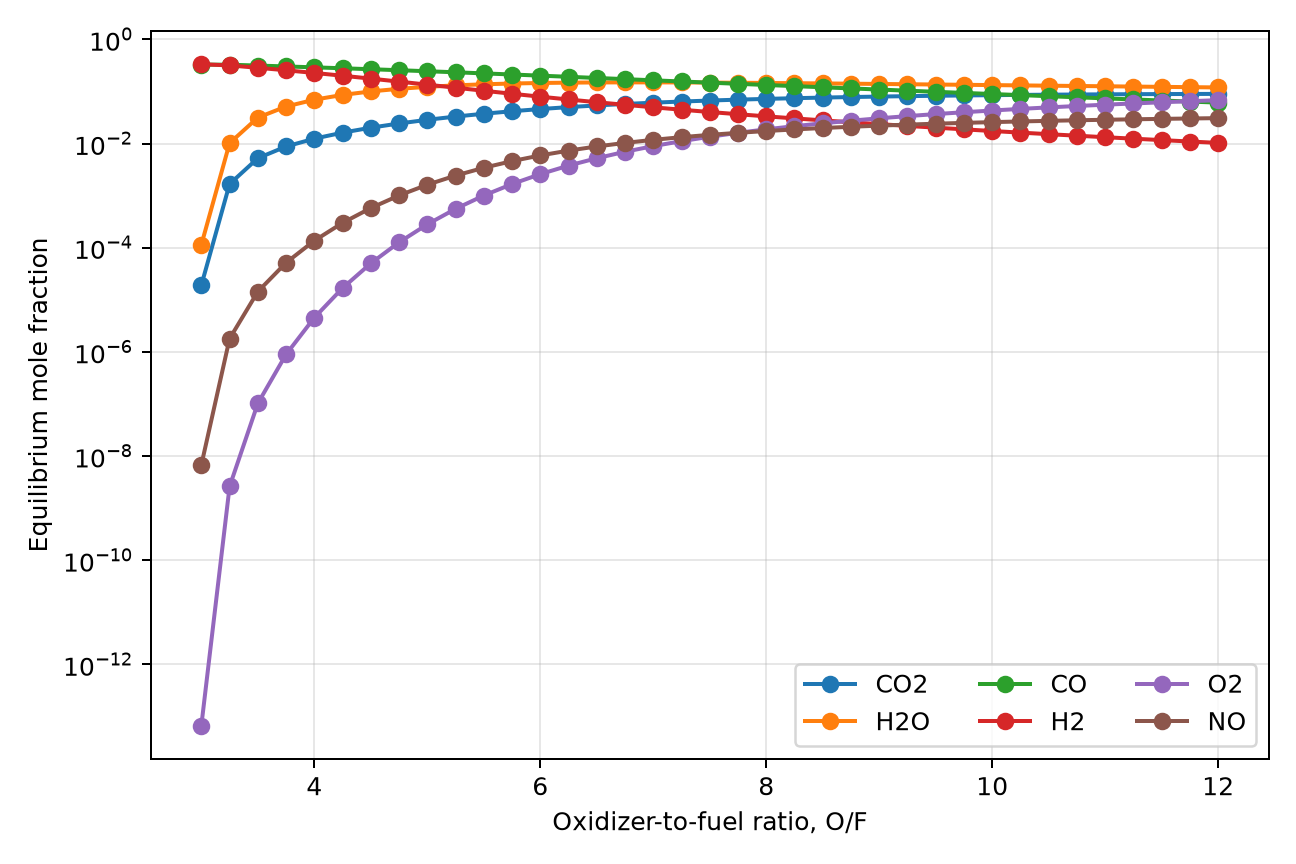
\includegraphics[width=0.82\linewidth]{../figures/species_vs_of_20bar.png}
\caption{Selected equilibrium product mole fractions at 20 bar.}
\end{figure}
\newpage

% Page 7
\section{Rocket Performance Results}
Maximum $c^*$ at 20 bar is 1627 m/s at O/F = 5.25. Maximum vacuum specific impulse is 290.2 s at O/F = 5.50; maximum sea-level specific impulse is 164.2 s. These optima are richer than the temperature maximum because H2/CO-rich products have lower molecular weight.

\begin{figure}[H]
\centering
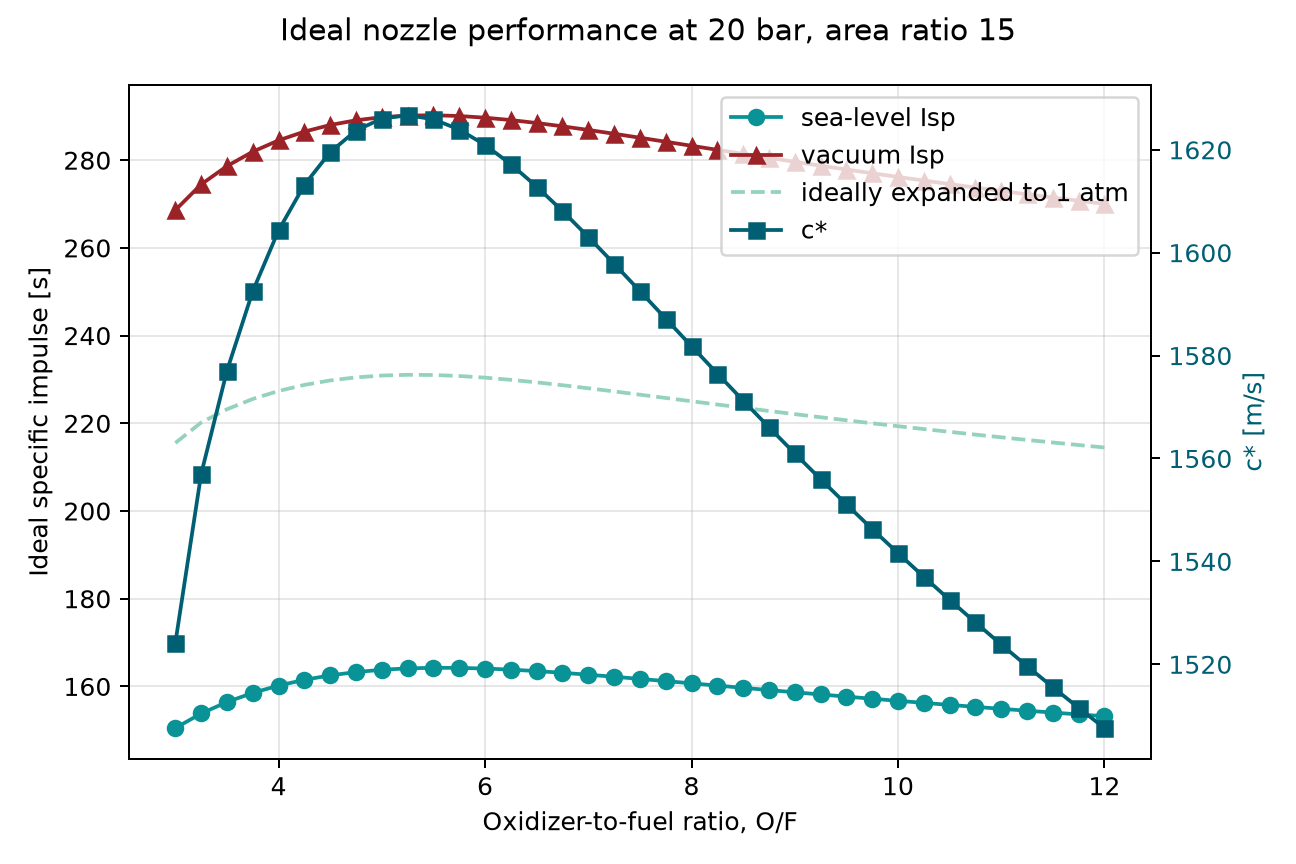
\includegraphics[width=0.82\linewidth]{../figures/performance_vs_of_20bar.png}
\caption{Fixed-area-ratio ideal nozzle performance and characteristic velocity at 20 bar.}
\end{figure}

\begin{tabular}{rrrrrr}
\toprule
O/F & T [K] & $\gamma$ & M [kg/kmol] & $c^*$ [m/s] & $I_{sp,vac}$ [s] \\
\midrule
4.00 & 2894 & 1.276 & 21.27 & 1604 & 284.5 \\
5.50 & 3279 & 1.257 & 23.71 & 1626 & 290.2 \\
6.00 & 3335 & 1.254 & 24.31 & 1621 & 289.7 \\
8.00 & 3379 & 1.249 & 25.95 & 1582 & 283.3 \\
10.00 & 3328 & 1.248 & 26.92 & 1542 & 276.2 \\
\bottomrule
\end{tabular}

\begin{figure}[H]
\centering
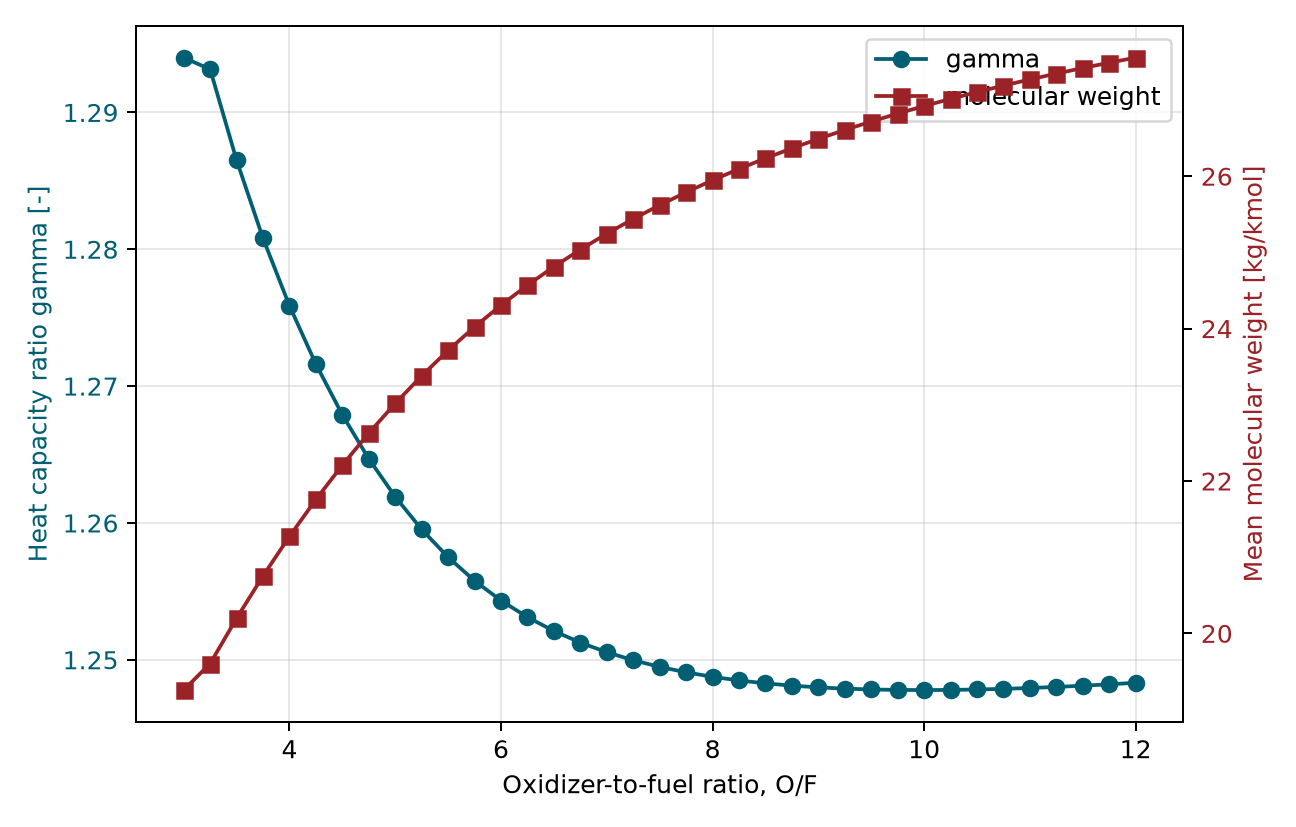
\includegraphics[width=0.76\linewidth]{../figures/gamma_molecular_weight_vs_of_20bar.png}
\caption{Heat-capacity ratio and mean molecular weight at 20 bar.}
\end{figure}
\newpage

% Page 8
\section{Pressure and Transport Results}
The pressure sweep is performed at O/F = 5.50. Raising pressure from 10 to 80 bar increases chamber temperature from 3219 to 3383 K and vacuum specific impulse from 287.9 to 294.2 s. Sea-level performance changes much more strongly because the fixed area-ratio nozzle is overexpanded at low pressure.

\begin{figure}[H]
\centering
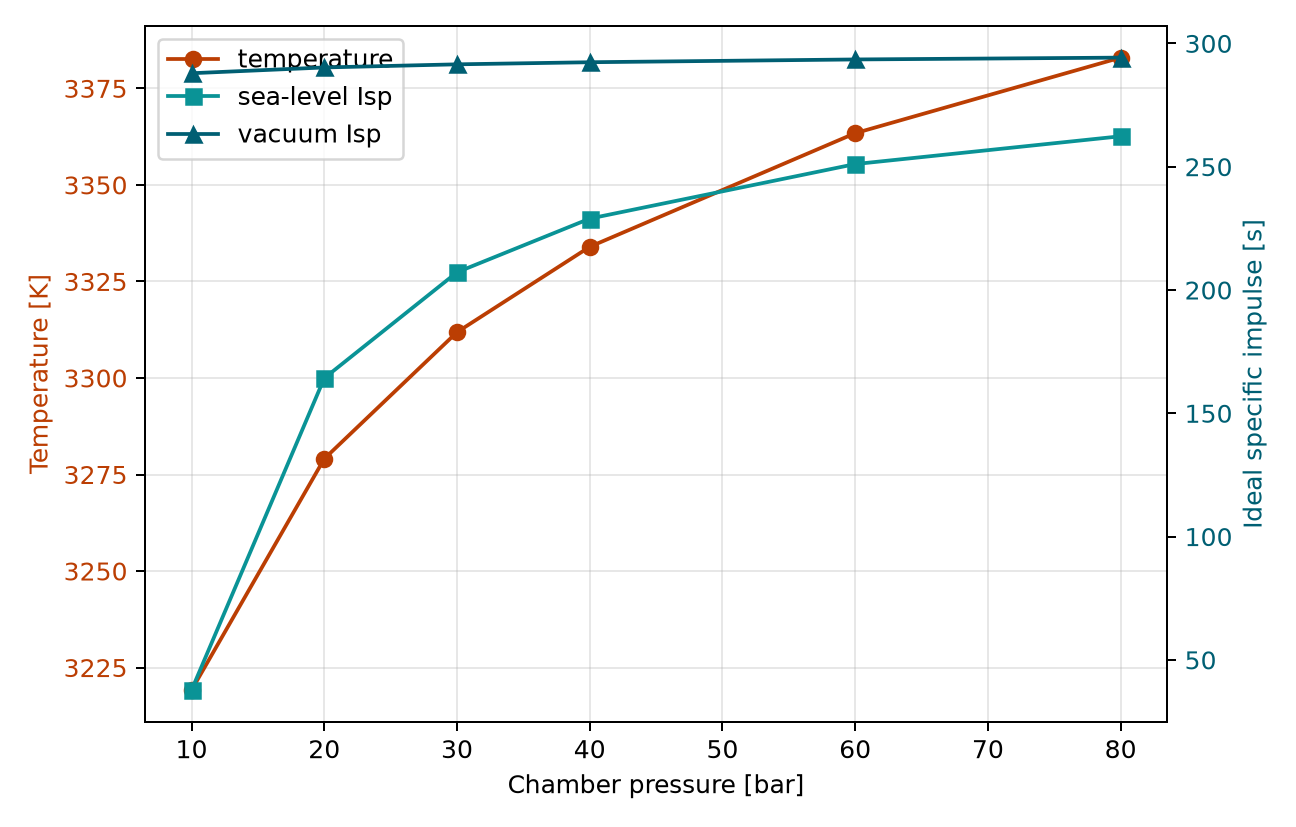
\includegraphics[width=0.82\linewidth]{../figures/pressure_sweep.png}
\caption{Chamber temperature and ideal specific impulse versus pressure.}
\end{figure}

Dynamic viscosity follows the temperature trend, while the Prandtl number varies more weakly. These quantities are recorded for future wall heat-transfer or cooling studies.

\begin{figure}[H]
\centering
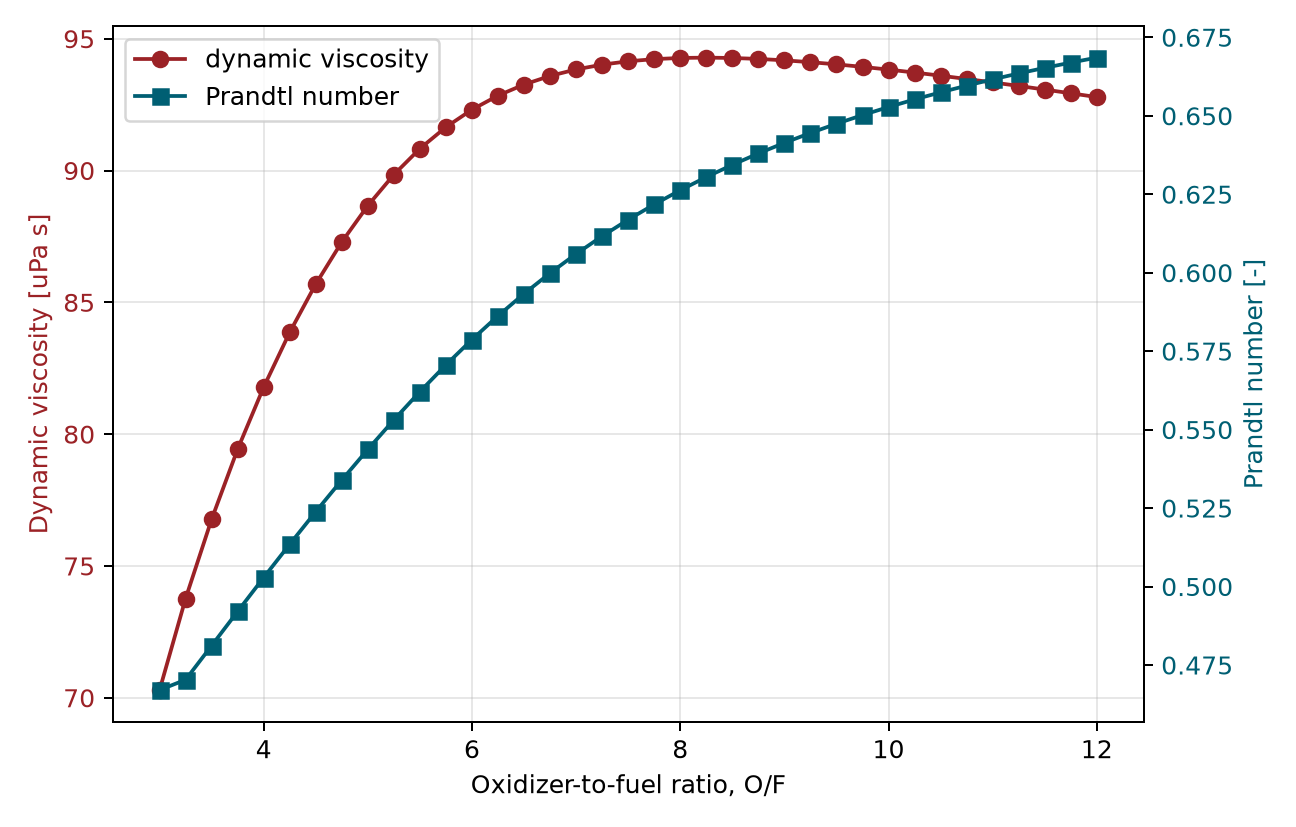
\includegraphics[width=0.82\linewidth]{../figures/transport_vs_of_20bar.png}
\caption{Dynamic viscosity and Prandtl number at 20 bar.}
\end{figure}
\newpage

% Page 9
\section{Hybrid Port Regression}
The illustrative model uses one cylindrical port, a 0.20 m grain, fuel density 900 kg/m3, and oxidizer mass flow 0.25 kg/s. Regression follows $\dot r=aG_{ox}^n$ with $a=7.0\times10^{-5}$ and $n=0.62$. During eight seconds, port diameter increases from 30.0 to 56.9 mm and O/F increases from 5.54 to 6.45. Interpolated ideal thrust decreases from approximately 669 to 650 N.

\begin{figure}[H]
\centering
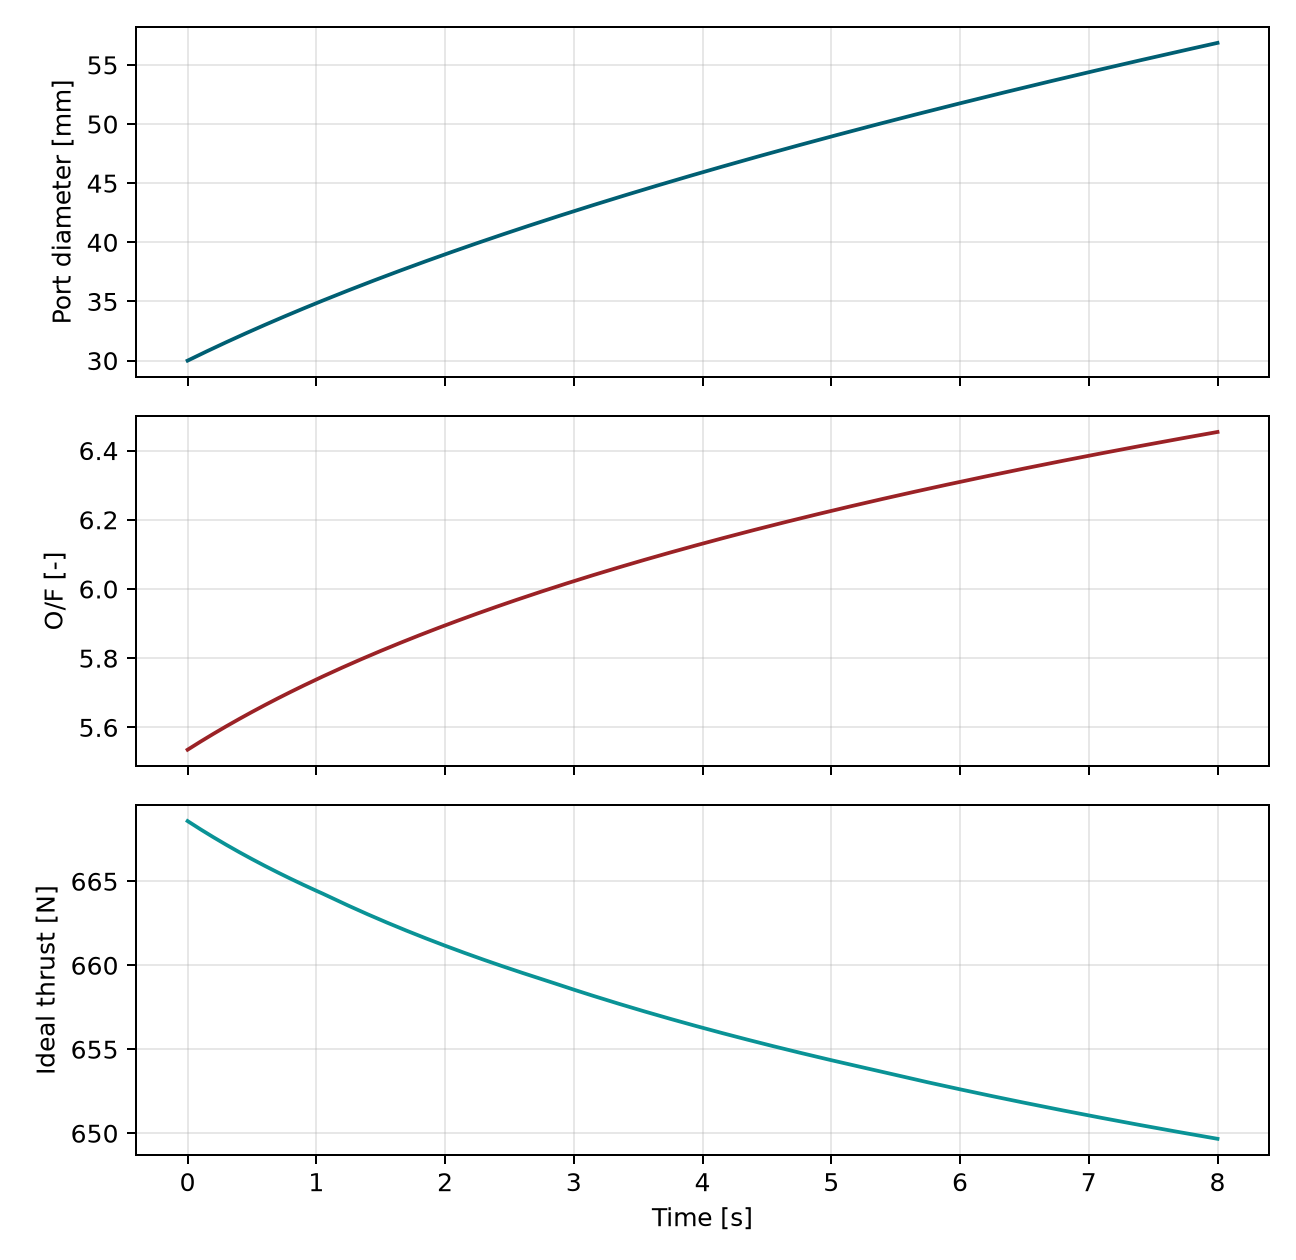
\includegraphics[width=0.64\linewidth]{../figures/port_regression_history.png}
\caption{Port diameter, O/F ratio, and interpolated ideal thrust.}
\end{figure}

\subsection{Limitations}
The main limitations are the ethylene fuel surrogate, gas-phase equilibrium, ideal reactant states, frozen-gamma nozzle expansion, fixed area ratio, no injector or chamber pressure-loss model, no wall heat transfer, no condensed carbon, and an illustrative regression coefficient. Some temperatures exceed the nominal 3000 K range of part of the mechanism data.

\subsection{Conclusions}
Maximum flame temperature is not the same as maximum rocket performance. At 20 bar, best $c^*$ and vacuum specific impulse occur around O/F = 5.25--5.50, far below stoichiometry. Pressure moderately improves vacuum performance but strongly changes sea-level expansion matching. O/F also moves during a burn, so thermochemistry, oxidizer flow, and grain geometry must be designed together.

\subsection*{References}
\small
[1] Cantera Developers, \url{https://cantera.org/}. [2] GRI-Mech 3.0, \url{https://combustion.berkeley.edu/gri-mech/}. [3] G. P. Sutton and O. Biblarz, \textit{Rocket Propulsion Elements}, Wiley. [4] M. J. Chiaverini and K. K. Kuo, \textit{Fundamentals of Hybrid Rocket Combustion and Propulsion}, AIAA. [5] S. Gordon and B. J. McBride, NASA RP-1311, 1994.

\end{document}
